\chapter{Background}

\label{Chapter2} 

\lhead{Chapter 2. \emph{Background}} 

\section{Native Client}
Native Client (NaCl) can be thought of as a new type of plugin for Google Chrome that allows binary programs to run natively in the web browser. It can be used as a `back end' for a normal web application written in JavaScript, since the binary program will run much faster. A NaCl module can be written in any language, including Assembly, so long as the binary is checked and verified to be safe by the NaCl sandbox \cite{nacl}. However, NaCl provides a Software Development Kit (SDK) that includes a compiler based on gcc that allows developers to compile C and C++ programs into binary that will work directly with the sandbox without further modifications. Thus, writing NaCl-compatible C++ programs is just as easy as writing normal C++ programs. The difference is that the sandboxes disallow unwanted side-effects, including system-calls. Since many applications might want to have these side effects, Native Client provides an Inter-Module Communications service (IMC) which allows modules to communicate with each other. The IMC service allows the use of the Pepper Plug-in API (PPAPI or `Pepper'), a convenient API that is bundled with the SDK. It can be used to do file IO, play audio, and render graphics. The Pepper API also includes the PostMessage functionality that we will use to implement Remote Procedure Calls between JavaScript and NaCl modules.

\subsection{NaCl Modules and the Pepper API}
A native client application consists of the following\cite{nacloverview}:
\begin{description}
  \item[HTML/JavaScript Application] 
  This is where the user interface of the application will be defined, and the   JavaScript here could also perform computations. The HTML file will include   the NaCl module by using an embed tag, e.g. \\
   \verb+<embed src="myModule.nmf" type="application/x-nacl" />+
  \item[Pepper API] 
  Allows the NaCl module communicate with the web browser and use its features.   Provides PostMessage to allow message passing to the JavaScript application.
  \item[Native Client Module] 
  The binary application, which performs heavy computation at native speeds.
\end{description}

\subsection{Communicating with JavaScript using postMessage}
The HTML5 postMessage API was designed to allow web workers to communicate with the main page's JavaScript execution thread. The JavaScript object is copied to the web worker by value. If the object has cycles, they are maintained as long as the cycles exist in the same object. This is known as the structured clone algorithm (need reference). 

In a similar way, postMessage allows message passing to and from NaCl modules. However, sending objects with cycles will cause an error. NaCl allows sending and receiving primitive JavaScript objects (Numbers, Strings, Booleans, null) as well as dictionaries (key-value Objects), arrays, and ArrayBuffers. ArrayBuffers are a new type of JavaScript object based on Typed Arrays \cite{typedarraysw3c} that allows the storing of binary data. Another key difference is that message types need to be converted into the correct type on the receiving end. For example, sending a JavaScript Object should translate into a dictionary type. Type conversions are quite subtle. The JavaScript types are very dynamic in nature. A JavaScript Number object could be an integer, a float, a double, `infinity', exponential, and so on. Sending C++ data to JavaScript is simple since it is converting from a more specific type to a less specific type (e.g. from `int' in C++ to `Number' in JavaScript). But converting from a JavaScript type to a C++ type requires more thought. The C++ Pepper API provides several functions to determine the JavaScript type (e.g. \verb+bool is_double()+), then we can extract and cast the data into our required type, also using Pepper (e.g. \verb+double AsDouble()+). From there, we can use the standard C++ type to perform the required computations.


\section{Remote Procedural Call (RPC)}
\label{RPCBackgroundSection} 
RPC is used to uniformly call a procedure that is on a different machine, or on the same machine but on different processes. RPC is implemented on top of a transmission protocol and should work regardless of the communication method we decide to use. For example, we could use TCP/IP for network communications, or any Inter-Process Communication (IPC) method if the caller and callee are on the same machine but in different processes. Normally, remote procedural call implementations would consist of the following steps, as shown in figure \ref{fig:rpc-components}.

\begin{enumerate}
  \item The caller code is written normally, and so is the server code, but the stubs are automatically generated using interface definition files (which we explain later in ...)
  \item When the remote call is made, it calls the user stub which packs the parameters and function call information into a packet.
  \item The packet gets transferred to its destination (either across the network as in figure \ref{fig:rpc-components}, or across the processes on the same machine using IPC). This is done through the RPCRuntime, which is a library that works on both ends (caller and callee) to handle communication details.
  \item The packet is received at the callee end by the RPCRuntime. It is then passed on to the server stub.
  \item The arguments and function call information are unpacked and a normal call is made to the actual procedure.
  \item When the procedure returns, it is passed back to the server stub where it is packed and transmitted back to the caller, which unpacks it and uses the result.
\end{enumerate}

\begin{figure}
    \centering
    % 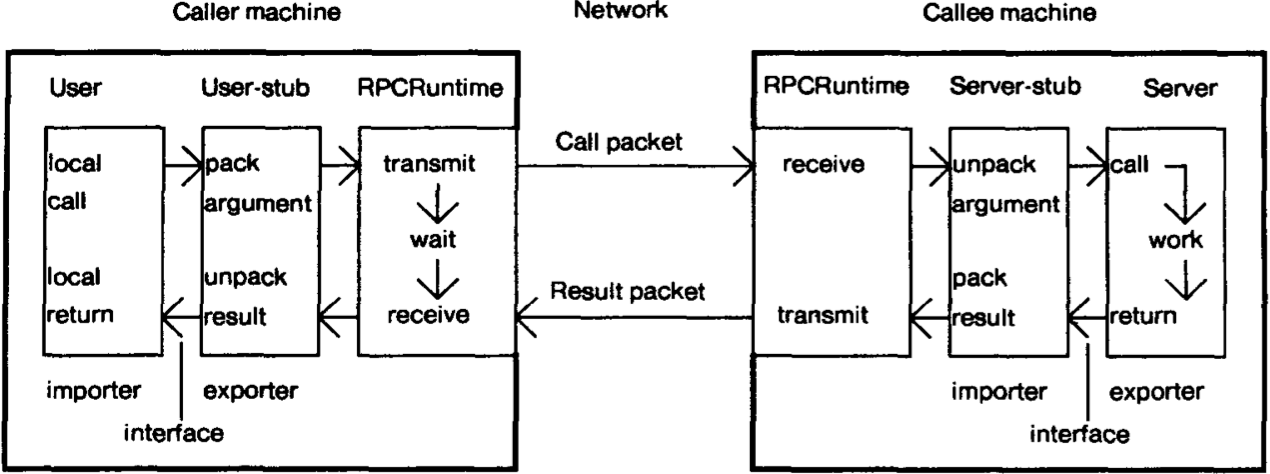
\includegraphics[width=\textwidth]{RPCDiagram_ImplementingRPC_ADBirrell_BJNelson.png} %uncomment to enable image
    \caption{The basic components of an RPC framework, from \cite{birrell1984implementing}}
    \label{fig:rpc-components}
\end{figure}

\subsection{The role of the RPCRuntime}
\label{RPCRuntimeBackgroundSection} 
The RPCRuntime is responsible for carrying out the actual communication of the RPC call information between the caller and the callee. It exists both in the caller and callee endpoints. When the caller makes a RPC call, the information is sent from the RPCRuntime sitting in the caller side, and is received by the RPCRuntime in the callee side. When the callee returns, the return data is sent from the callee's RPCRuntime to the caller's RPCRuntime.

In order to keep the context of a remote call, the RPCRuntime also sends some extra meta data along with the arguments. This meta data includes: 

\begin{enumerate}
	\item A call identifier. This is used for two reasons:
	\begin{enumerate}
		\item To check if the call has already been made (i.e. to ensure no duplicate calls)
		\item To match the return value of the callee with the correct caller.
	\end{enumerate}
	\item The name of the procedure the caller is calling.
	\item The arguments (parameters) we wish to pass to the remote procedure.
\end{enumerate}

The RPCRuntime on the caller side maintains a store of call identifiers that are currently in progress. When the remote functions return, they send the same call identifier along with the return value. That call identifier is then removed from the caller's store to indicate that the remote call has completed.


\section{Open Network Computing Remote Procedure Call}
\label{ONCRPCBackgroundSection} 
Open Network Computing (ONC) is a suite of software originally developed by Sun Microsystems. It provides a Remote Procedure Call (RPC) system along with an External Data Representation (XDR) format used alongside it. The ONC RPC system implements some tools and libraries that make it easy for developers to specify and use remote functions. These are:

\begin{enumerate}
	\item \textbf{RPCGen Compiler:} As mentioned earlier, the role of the user and server stubs is to pack and unpack arguments and results of function calls. To pack the arguments, the stub looks at the argument types and matches them with the number of arguments and their types of the server (callee) function definition. Thus, the stubs need to be written with knowledge of the interface of the actual procedures that will be called. We can define these interfaces in an abstract way, so that we could generate these stubs automatically even if the languages used in the different endpoints are different. In ONC RPC and many other systems, this abstract representation is in the form of an Interface Definition Language (IDL) file. When we pass the IDL file into the RPCGen compiler, it automatically generates the stubs we need to perform remote procedure calls.
	\item \textbf{XDR Routines:} These convert the types of the parameters and return values to and from the external data representation. XDR routines exist for many C types, and the system allows you to write your own XDR routines for complex types.
	\item \textbf{RPC API library:} This is an implementation that fulfils the role of the RPCRuntime described in \ref{RPCRuntimeBackgroundSection}. It provides a set of API functions that set up the lower level communication details, binding, and so on.
\end{enumerate}

Remote procedures in ONC RPC are identified by a program number, a version number, and a procedure number. There also exists a port mapper that map the program number to a port, so that several programs can run on the same remote machine. 

\subsection{Interface Definition Language files}
In ONC RPC, the XDR is used to define RPC definitions. For example, the RPC definition in listing \ref{samplerpc} defines an interface for a simple function that takes in a character string  and returns a structure containing two fields. As discussed in \ref{ONCRPCBackgroundSection}, we can see the program number is \verb+80000+ and the procedure number of the \verb+generate_keypair+ function is \verb+1+.

\lstset{language=c,caption={An example RPC definition for a key-pair generator function},label=samplerpc}
\begin{lstlisting}
/* File: keypairgen.x */
struct key_pair_t
{
  string  public_key<500>;
  string  private_key<500>;
};

program KEYPAIRGEN_PROGRAM
{
  version KEYPAIRGEN_VERSION
  {
    /* Produce a public/private key pair using a passphrase  */
    key_pair_t generate_keypair (string) = 1;
  } = 0;
} = 80000;
\end{lstlisting}

We can use the RPCGen compiler to then create client and server stubs. Passing the definition file \verb+keypairgen.x+ (shown in listing \ref{samplerpc}) into \verb+rpcgen+ will produce the following files:

\begin{itemize}
	\item \textbf{keypairgen.h} The header file, which would be included in both client and server code. Includes the actual C definition of the result\_t structure we defined in the XDR.
	\item \textbf{keypairgen\_clnt.c} The client stub, which packs the parameters and uses the RPC API library to execute the actual remote procedure call.
	\item \textbf{keypairgen\_svc.c} The server stub, which uses the RPC API to set up a listener for RPC calls. RPC calls are received, parameters are unpacked, and the actual function implementation (of \verb+generate_keypair+) is called.
	\item \textbf{keypairgen\_xdr.c} Defines methods for packing more complex structures, such as the \verb+key_pair_t+ structure we defined.
\end{itemize}

Now we need to write the actual implementation of the RPC procedure we wish to call remotely, namely \verb+generate_keypair+. This will include the generated header file and follow the specification we defined, as shown in listing \ref{samplerpcImp}. \\


\lstset{language=c,caption={An example server-side implementation of the procedure defined in \ref{samplerpc}},label=samplerpcImp}
\begin{lstlisting}
#include "keypairgen.h"

key_pair_t *
generate_keypair_0_svc(char **argp, struct svc_req *rqstp)
{
  static key_pair_t  result;
  // TODO: Actual implementation
  return(&result);
}
\end{lstlisting}

Finally, we call the remote procedure from the client, which includes the same header file and simply calls \verb+generate_keypair_0+, passing in the string parameter.



\section{WebIDL}


